\section{Introduction}
\label{sec:introduction}

Future Cyber-Physical Smart Power Grid~\cite{huang11} system should have embedded computing devices that monitor and control distributed generation, storage and power transfers while also maintaining safety, reliability and efficiency in a secure manner. Maintaining stability and correctness of all the components in CPS is a major challenge. Compensating for stability or correctness in one component is reflected in other components. For example, incorrect actions taken in physical domain can cause network to go unstable. Therefore, it is crucial to have correct scheduling of actions in domains to ensure the overall system stability.

% Invariant technique Vs. Other techniques
Although there are methodologies that consider one or two components of a system and compose stability, such as switched-systems theory~\cite{donkers11} that models stability of a plant, Hybrid automata~\cite{henzinger96}, timed I/O automata~\cite{alur94} that represents a mix of continuous and discrete states in verification process~\cite{chutinan03,tomlin03}, our framework of composing components with stability in CPS is based on $invariants$ technique. Figure~\ref{fig:invariant_conjunction} shows the composition of cyber, physical, network and scheduling components through conjunction of logical invariants, where overall system stability and correctness is expressed in the form of invariants ($I_{C1} \wedge I_{C2} \wedge I_{Cn}$). This approach is not only limited to smart grid design, but can also be generalized to different cyber-physical systems with different functionalities. The scheduling domain in Figure~\ref{fig:invariant_conjunction} refers to scheduling of power transfer messages between smart-grid nodes over the communication network. Thus, "Network" and "Scheduling" being tightly coupled, are depicted forming one invariant in Figure~\ref{fig:invariant_conjunction}. In this paper, we insist scheduling of actions (power messages) at \textit{appropriate} times such that the system stability is maintained, rather than performing actions at pre-defined intervals as done in traditional real-time scheduling. In Cyber-Physical smart grid system, stability and state of a physical system depends on, state of the communication network carrying power migrate messages and power migrate acknowledgment messages between the nodes. Therefore, state and stability of communication network is also affected by number of outstanding (in transit) power migrate messages.

\begin{figure}[htb]
  \begin{center}
%    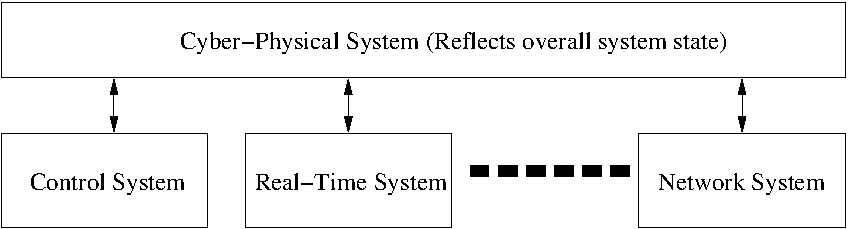
\includegraphics[width=0.45\textwidth]{Figures/cps-n-domains.pdf}
     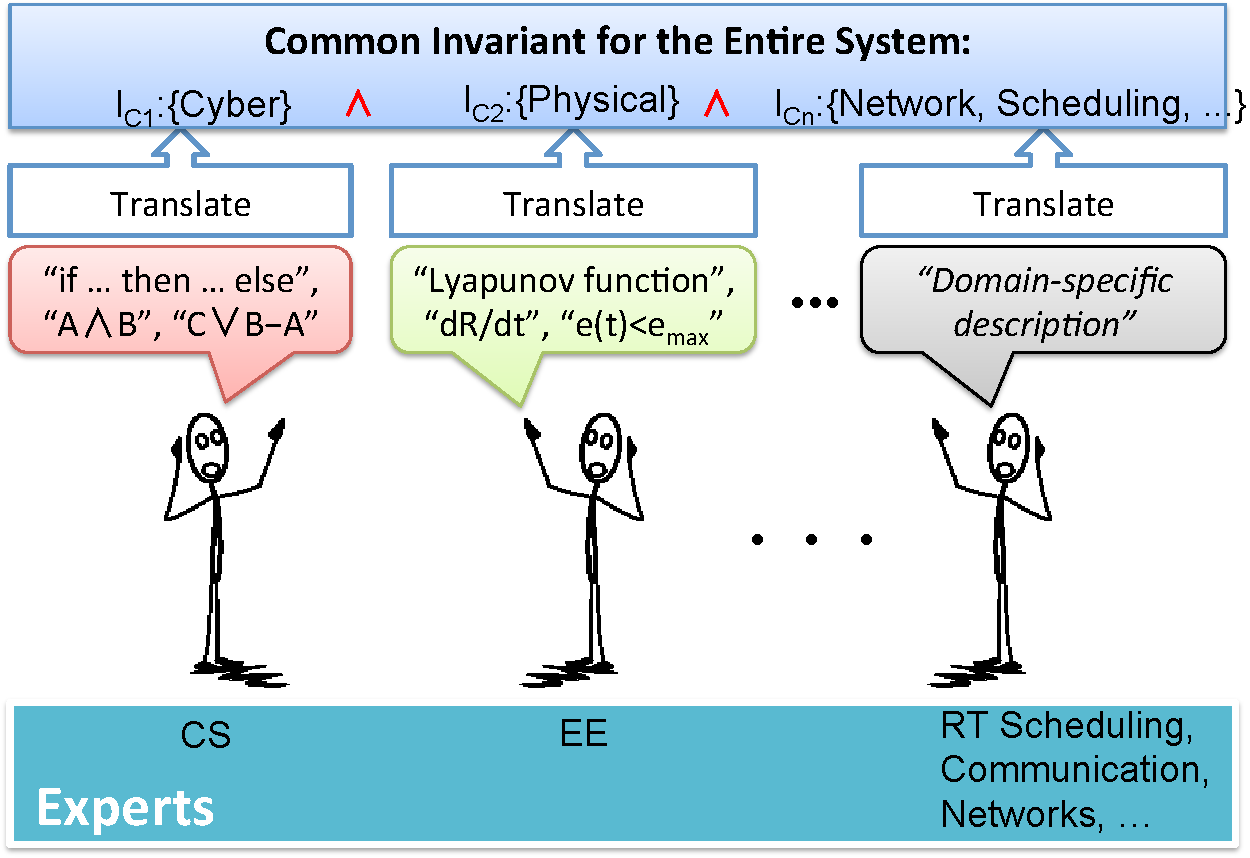
\includegraphics[width=0.9\columnwidth]{Figures/Invariant_Overview.pdf}
  \caption{Overview of invariant-based approach}
  \label{fig:invariant_conjunction}
  \end{center}
\end{figure}

In recent work~\cite{acsmartgrid}, we developed a 
scheduling invariant for our distributed, adaptive algorithm for scheduling power 
migrations between smart grid nodes and demonstrated that conjunction of such a
scheduling invariant and an invariant for physical system state is necessary to 
maintain overall system stability. In order to improve efficiency along with stability, components in CPS must have certain amount of inter-component information. In the current paper, we focus on 
improving the efficiency while also maintaining the stability of smart grid nodes 
by exploiting the network congestion information obtained from Early Congestion 
Notification (ECN) scheme. In this scheme, packets are marked indicating impending congestion,
instead of dropping them\cite{floyd1994tcp, ramakrishnan1999proposal, 
ramakrishnan2001addition}. We allow the smart grid nodes to sense the possible 
upcoming network congestion and change the amount of power being transferred with 
every power migrate message in order to compensate for reduced rate of power transfers.
As of our knowledge, this is the first work that explore ECN scheme from CPS context
for the benefit of physical system efficiency as well as take necessary action to 
reduce network congestion.

The rest of this paper is organized as follows. Section \ref{sec:related_work}
provides some background information and discusses related work. We present our
system model and assumptions in Section \ref{sec:assumptions}. Section
\ref{sec:invariants} presents our physical system 
invariant and adaptive scheduling invariant. Section \ref{sec:power_management_algo} 
presents our resulting power management algorithm. Our simulation setup is introduced 
in Section \ref{sec:simulation_setup} and results are presented in Section
\ref{sec:results}. Section \ref{sec:discussion} presents a brief discussion and
conclusions are presented in Section \ref{sec:conclusions}.

